%%%%%%%%%%%%%%%%%%%%%%%%%%%%%%%%%%%%%%%%%%%%%%%%%
%
% Universita' degli Studi dell'Insubria
% Template LaTeX realizzato da Nicola Landro
%
%%%%%%%%%%%%%%%%%%%%%%%%%%%%%%%%%%%%%%%%%%%%%%%%%
\documentclass[a4paper, 11pt, twoside]{book} % twoside, oneside
\usepackage[a4paper]{geometry}
\usepackage[italian]{babel}
\usepackage{textcomp}
\usepackage{color}
\usepackage{url}
\usepackage{amsfonts}
\usepackage{float}
\usepackage{booktabs}
\usepackage{longtable}
\usepackage{makeidx}
\usepackage{fancyhdr}
\usepackage[times]{quotchap}
\usepackage{multirow}
\usepackage{version}

\usepackage{listings}
\usepackage{color}
\definecolor{gray}{rgb}{0.9,0.9,0.9}
\definecolor{orange}{rgb}{0.9,0.5,0.08}
\definecolor{purple}{rgb}{0.5,0.01,0.5}


%%Stile per codice

\lstdefinestyle{customjava}{
  	language=Java,
  	frame=tlrb,
  	aboveskip=3mm,
  	belowskip=6mm,
  	showstringspaces=false,
  	columns=flexible,
  	basicstyle={\small\ttfamily},
  	numbers=left,
    numberstyle=\tiny\color{orange}\ttfamily,
    numbersep=5pt,
  	keywordstyle=\color{purple},
  	commentstyle=\color{orange},
  	stringstyle=\color{blue},
  	breaklines=true,
  	breakatwhitespace=true
  	tabsize=3
}


%% Aggiunge una linea al di sotto di ogni sezione principale
\usepackage[calcwidth]{titlesec}
\titleformat{\section}[hang]{\sffamily\bfseries}
 {\Large\thesection}{12pt}{\Large}[{\titlerule[0.4pt]}]

%% Gestisce la grafica a seconda che si usi latex o pdflatex
\newif\ifpdf
\ifx\pdfoutput\undefined
\pdffalse % no pdflatex
\else
\pdfoutput=1 % pdflatex
\pdftrue
\fi
%
\ifpdf
\usepackage[pdftex]{floatflt,graphicx}
\DeclareGraphicsExtensions{.pdf,.mps,.png,.jpg}
\usepackage[pdftex]{hyperref}
\else
\usepackage{floatflt,graphicx}
\DeclareGraphicsExtensions{.eps}
\fi
\usepackage{subfigure}

%\usepackage{algorithm}
%\usepackage{algorithmic}
\usepackage[utf8]{inputenc} % per accenti

%%tabella con linee colorate
\usepackage{colortbl}

%%%%%%%%%%%%% NUOVI COMANDI E IMPOSTAZIONI %%%%%%%%%%%
\newenvironment{mcquote}
  {\begin{list}{}{
      \setlength{\rightmargin}{\leftmargin}}
         \item[]``\ignorespaces}
  {\unskip''\end{list}}
  
\newcommand{\mcchap}[2]{\protect{
 \chapter{#1}
 \label{#2}
}}

%% Gestione header: no header sulle dispari bianche
\makeatletter
\def\cleardoublepage{\clearpage\if@twoside \ifodd\c@page\else%
    \hbox{}%
    \thispagestyle{empty}%              % Empty header styles
    \newpage%
    \if@twocolumn\hbox{}\newpage\fi\fi\fi}
\makeatother

\newcommand{\codice}[1]{\protect\texttt{\small{#1}}}

\newcommand{\mcproc}[1]{\ensuremath{\mbox{\sc #1}}}

\newcommand{\mctodo}[1]{\protect{
  \bigskip
  \begin{tabular}{|p{13cm}} \textcolor{red}{\underline{TODO:}} \small{#1} \end{tabular}}
}

\newcommand{\mcnota}[1]{\protect{
  \bigskip
  \begin{tabular}{|p{13cm}} \underline{NOTA:} \small{#1} \end{tabular}}
}

\makeindex
\linespread{1.1}
%\floatname{algorithm}{Algoritmo}
%\renewcommand{\listalgorithmname}{Elenco degli algiritmi}



%%%%%%%%%%%%%%%% METADATI DOCUMENTO %%%%%%%%%%%%%%%%%%
\date{}

%%%%%%%%%%%%%%%%%% INIZIO DOCUMENTO %%%%%%%%%%%%%%%%%%
\begin{document}
\pagestyle{empty}

%% Pagina del titolo
  \begin{titlepage}
  \begin{center}
  \begin{large}
  {\fontsize{20.74}{18}\selectfont\vspace*{0.50cm}Universit\`a degli Studi dell'Insubria}\\
  Facolt\`a di Scienze MM.FF.NN.\\
  Corso di Laurea Triennale in Informatica
  \end{large}
  
  \vspace{1cm}
  \begin{figure}[h]
    \begin{center}
      
\includegraphics[scale=0.25]{copertina/logounivector.pdf}
    \end{center}
  \end{figure}

    {\fontsize{26}{26}\usefont{OT1}{phv}{m}{n}\selectfont\par\vspace*{0.75cm}
    Ristutturazione di un sistema
    \vspace{.15em}di gestione dei contenuti}
    \par
    
    \vfill
    \vspace{3cm}
    \begin{large}
    Relatore: Dott. Ignazio Gallo\\

    \vspace{1.0cm}
    Tesi di Laurea di\\
   Matteo Franceschi De Marchi\\
    Matricola 325680\\
    \vspace{0.5cm}

    \end{large}

    Anno Accademico 2016-2017

  \end{center}
\end{titlepage}


%% Dedica
\frontmatter{}
  \begin{flushright}
    \vspace*{0cm}
    \vfill
    \textit{ 
      ``What a liberation to realize that the “voice in my head” is not who I am. Who am I then? The one who sees that.''- Eckhart Tolle
    }
    \vspace{2.5cm}
  \end{flushright}
  \cleardoublepage
  
%% Indice ed elenchi
  
  \pagenumbering{roman}
  \setcounter{page}{1}
  \setcounter{tocdepth}{2}
  \tableofcontents
  \listoffigures
  \listoftables
%% Inizio capitoli
  \mainmatter{}
  
%% Capitoli
  \pagestyle{fancy}
  \renewcommand{\chaptermark}[1]{\markboth{#1}{}} 
  \renewcommand{\sectionmark}[1]{\markright{\thesection\ #1}} 
  \fancyhf{} % delete current setting for header and footer 
  \fancyhead[LE,RO]{\bfseries\thepage} 
  \fancyhead[LO]{\bfseries\rightmark} 
  \fancyhead[RE]{\bfseries\leftmark} 
  \renewcommand{\headrulewidth}{0.8pt} 
  \renewcommand{\footrulewidth}{0pt} 
  %\renewcommand{\headheight}{16pt}
  \addtolength{\headheight}{0.5pt} % make space for the rule 
  \fancypagestyle{plain}{% 
  \fancyhead{} % get rid of headers on plain pages
  \fancyfoot[C]{\bfseries \thepage}
  \renewcommand{\headrulewidth}{0pt} % and the line 
  } 

  \cleardoublepage{}
  \setcounter{page}{1}
  
%-------------------------------------------------------------
%				INTRODUZIONE
%-------------------------------------------------------------

\mcchap{Introduzione}{cap:intro}

Nel periodo di apprendistato in 7Pixel sono stato assegnato al team Iguana, team che si occupa
della gestione principalmente front-end dei siti del \emph{Kirivo Network}

\section{Il Kirivo Network}
Il Kirivo Network (KN) è attualmente composto da due siti  \url{www.kirivo.it} 
e \url{www.origini.it}:

\url{www.kirivo.it} è un negozio online che vende prodotti di tutte le categorie.
Il marketplace dispone di un offerta di oltre 800.000 articoli in tutte le categorie tra cui
elettrodomestici, prodotti per la casa, smartphone e TV, giocattoli, moda e altri.

\url{www.kirivo.it} è il marketplace ufficiale di \url{www.trovaprezzi.it}, il principale motore
di ricerca italiano per la comparazione di prezzi.

\url{www.origini.it} è una divisione verticale di Kirivo. Il sito è specializzato nella vendita
di vini e offre un ampia offerta di prodotti divisi per cantine e regioni. Il sito
è online da Novembre 2016.

I siti del Kirivo Network fanno utilizzo di servizi di Back-End comuni che permettono 
di effettuare acquisti nei due siti utilizzando un unico account ed un unico carrello.

Con buone probabilità verranno aggiunti in futuro nuovi siti verticali per alcune categorie
di Kirivo.

\section{Architettura del Kirivo Network}
Per l'erogazione dei siti del Kirivo network vengono usati diversi server:
\begin{itemize}
\item {\bf Hybris}: una piattaforma Enterprise di e-commerce scritta in Java che offre una soluzione all-in-one per i siti 
di e-commerce comprendendo servizi quali la gestione del catalogo dei prodotti, degli utenti e la 
gestione sicura dei pagamenti. La scelta di utilizzare una piattaforma di e-commerce a pagamento è stata fatta
principalmente per velocizzare i tempi di sviluppo in fase iniziale.

Hybris utilizza una database relazione Postgres e il suo cataologo viene indicizzato dal motore di ricerca SolR.

\item {\bf SolR}: un motore di ricerca scritto in Java che permette di indicizzare i prodotti presenti a catalogo per una accesso
più rapido.

Permette inoltre di filtrare in modo efficente i prodotti presenti a catalogo ottimizzando
le ricerche per categorie o caratteristiche del prodotto.

\item {\bf Kiruby}: un web-server Ruby che eroga le pagine web dei siti, si interfaccia con Hybris, Solr e Kitty utilizzando i loro
servizi di backend. 
\item {\bf Wordpress}: usato per la creazione di pagine di contenuto che vengono incluse da Kiruby.

Il server di Wordpress si trova nella LAN aziendale e si interfaccia solamente con il server Kiruby, la sua
presenza è nascosta agli utenti finali.
\item {\bf Redis}: un database noSql che, salvando tutto il suo contenuto in RAM, garantisce alte prestazioni.

Viene usato da Kiruby come cache di contenuti, specialmente per le richieste di Kiruby a Wordpress.

\item {\bf Nginx}: un Reverse proxy usato per redirigere le chiamate fatte ai domini \url{www.kirivo.it} 
e \url{www.origini.it} ai server opportuni.
\end{itemize}

\begin{figure}
  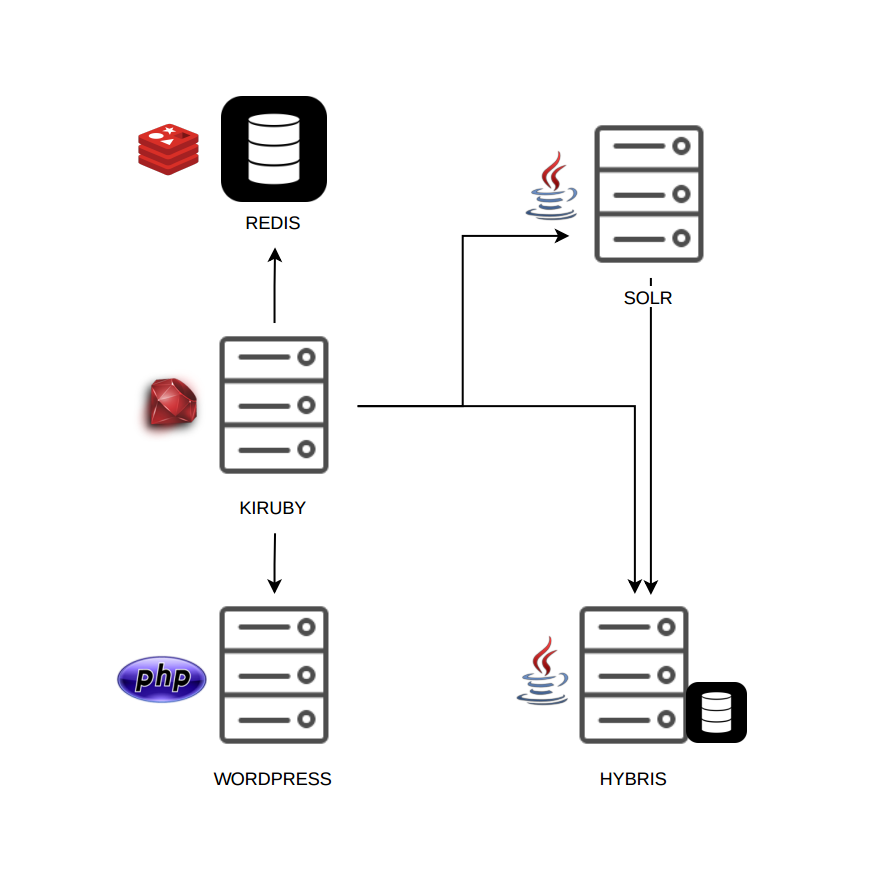
\includegraphics[width=\textwidth]{figure/arch.png}
  \caption{Schema dell'architettura del Kirivo Network.}
  \label{fig:kn}
\end{figure}


\newpage

\section{I team del Kirivo Network}
Lo sviluppo è l manutenzione dei siti del Kirivo Network viene effettuato da più team e questi sono:
\begin{itemize}
\item {\bf Team Iguana}: si occupano dello sviluppo di Kiruby.
\item {\bf Team Nimbus}: si occupano dello svliuppo di Hybris SolR e Kitty.
\item {\bf Content Manager}: si occupano della comunicazione con i venditori, della gestione dei prodotti a catologo
 e della creazione di pagine di speciali, lavorano interfacciandosi con Hybris e Wordpress.
\item {\bf Grafica}: lavora o direttamente su Kiruby o da al team Iguana grafiche HTML che vengono poi rese dinamiche 
ed integrate con i vari servizi.
\end{itemize}

\section{Gestione delle homepage} 	

Le homepage di Origini e Kirivo sono le pagine che, nei rispettivi siti, possono cambiare contenuto più 
frequentemente. Inoltre scegliere quali prodotti, quali offerte e quali contenuti 
vanno inseriti in homepage non è compito dei programmatori ma dei \emph{content managers},
quindi si rivela importante dare la possibilità ai \emph{content} di fare modifiche, come cambiare un prodotto da
mettere tra quelli in evidenza in homepage, o il testo di un pannello con la cantina del mese senza dover passare 
dai programmatori per fare modifiche.

Per dare più libertà ai \emph{content}, il contenuto della homepage, ovvero tutto quello che non è
header e footer, non si trova nel server Kiruby ma in pagine Wordpress che i content possono direttamente 
modificare accedendo alla sezione admin di Wordpress.

\begin{figure}
  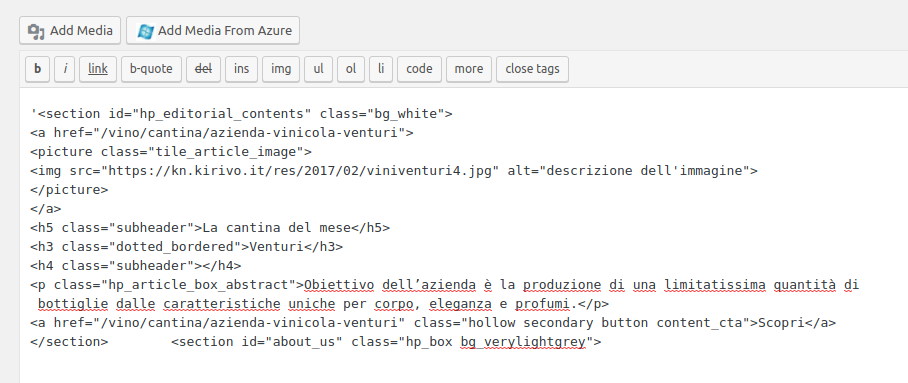
\includegraphics[width=\textwidth]{figure/whtml.png}
  \caption{L'interfaccia visualizzata dai content managers per modificare la pagina.}
  \label{fig:whtml}
\end{figure}

\begin{figure}
  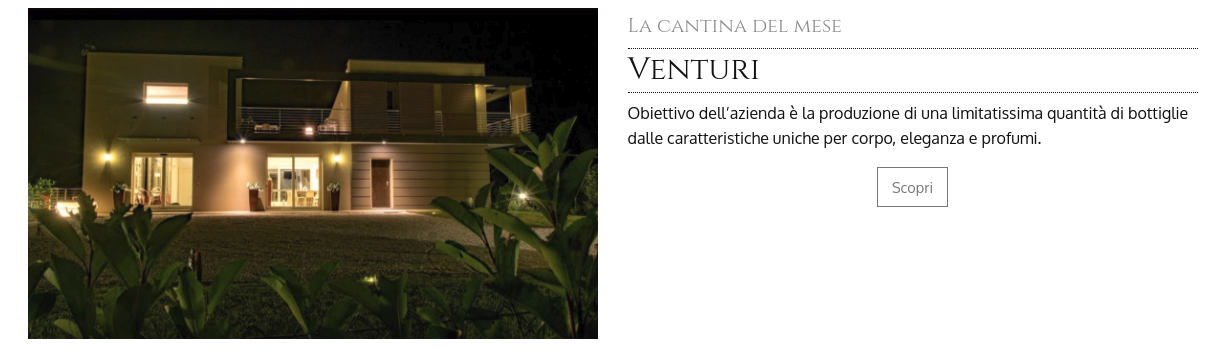
\includegraphics[width=\textwidth]{figure/wrender.png}
  \caption{Risultato renderizzato della componente compilata in figura \ref{fig:whtml}.}
  \label{fig:wrender}
\end{figure}


\newpage

Il server Kiruby quando deve riceve una richiesta per la homepage chiede a Wordpress la sua pagina della home, ne estrae
il contenuto e lo renderizza nell'HTML che restituisce. Il contenuto di Wordpress viene incluso nell'HTML tra Header e Footer il cui codice invece resta in Kiruby, in comune a tutte le altre pagine.


\begin{figure}
  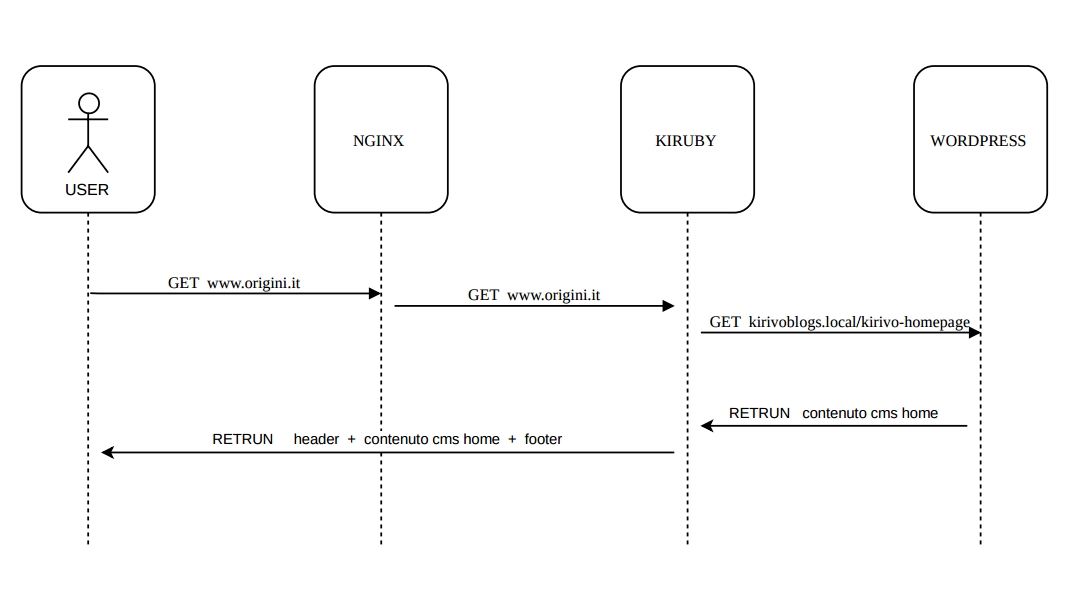
\includegraphics[width=\textwidth]{figure/homeseq.png}
  \caption{Funzionamento della richiesta della homepage.}
  \label{fig:homeseq}
\end{figure}



\section{La gemma cmsdealer}
Per visualizzare contenuti dinamici, come ad esempio un Box di 4 vini viene utilizzata
una gemma Ruby chiamata \emph{cmsdealer}.

La gemma è necessaria per il fatto che le informazioni dei prodotti non sono accessibili a Wordpress, che viene utilizzato
come server per la gestione e la modifica di contenuti editoriali, ma sono accessibili a Kiruby che ha al suo interno diversi
meccanismi per accedere alle informazioni dei prodotti andandosi ad interfacciare con Hybris e SolR.

La gemma \emph{cmsdealer} usata dal server Kiruby scansiona la pagina di Wordpress da includere,
se incontra un tag di nome \emph{dynamic} ne legge l'attributo \emph{type} e in base al valore di questo
seleziona il corrispondente template, legge l'ID dei prodotti e sostiusice al tag \emph{dyanmic} l'HTML del box con
i valori dei prodotti selezionati

Esempio: se processando la pagina HTML di Wordpress Kiruby trova
\begin{verbatim}
	<dynamic type="OriginiListingBox" ids="3422,2345,2872,2209" />
\end{verbatim}
allora verrà cercato il template di \emph{originilistingbox.html.erb} e verrà popolato
coi valori dei prodotti con gli identificativi specificati nell attributo \emph{ids}.

% immagine meta sito metà wp-admin di prodotti in evidenza

\newpage
\section{Obbiettivo}
L'obbiettivo del progetto è quello di rendere l'edit delle pagine
da parte dei content molto più semplice e flessibile,
facendo in modo che i contenuti delle homepage possano essere editati visualmente e non
andando a mettere mano direttamente sul codice HTML.

Per farlo i content dovranno interagire con un interfaccia grafica web che permette
la modifica delle informazioni necessarie e di poter spostare e copiare
componenti della home con un click o con un drag and drop.

\section{Obbiettivo secondario}
Obbiettivo secondario del progetto e di rendere il sito più manutenibile.

La criticità del sistema è che contiene codice duplicato nella gemma CmsDealer, in Kiruby
e nei widget di Wordpress. 

Per risolvere il problema sono state create le  \emph{RenderdPricesAPI} 
che restituiscono frammenti di HTML renderizzato per varie componenti della home.

In questo modo il codice del template resta solamente in Kiruby e esponendo le 
API questo viene usato sia dai Widget di Wordpress sia dalla gemma CmsDealer

  
%-------------------------------------------------------------
%				AGILE
%-------------------------------------------------------------

\mcchap{Sviluppo agile}{cap:agile}

In 7Pixel si sviluppo utilizzando metodologie agili, il software viene sviuppato
iterativamente, nuove feature e aggiornamenti vengono pubblicati quotidianamente.

\section{TDD}
Una tecnica rigorosamente usata in azienda è il TDD Test Driven Development ovvero, prima di
aggiungere una qualsiasi nuova funzionalità si scrive un test che passa solo se 
quella funzionalità fosse implementata. 

Dopodichè si cerca nel modo più veloce e semplice possibile di fare passare il test

Una volta passato il test si fa del refactoring per rendere il codice più leggibile
e soprattutto manutenibile

\section{Pair Programming}
Tutti i lavori effettuati su Kiruby sono sempre stati fatti in Pair Programming
con un membro del team

Il Pair Programming si rivela molto efficace, perchè si riescono ad evitare molti
errori "di distrazione" che possono costare caro in termini di tempo e soprattutto
si ha molto spesso la possibilità di confrontarsi con punti di vista diversi che possono
portare ad un analisi più approfondita del problema e a soluzioni migliori 


  
%-------------------------------------------------------------
%				Studio in azienda
%-------------------------------------------------------------

\mcchap{Fase di formazione aziendale}{cap:agile}

Durante i primi due mesi di tirocinio, la maggior parte del mio tempo è stato speso in formazione,
il mio studio può essere diviso in tre argomenti principali:

\begin{itemize}
\item Tecnologie
\item Sviluppo agile
\end{itemize}

Lo studio dei primi due è stato prevalentemente pratico, mentre per lo sviluppo
agile lo studio è stato in gran parte teorico ma anche pratico

\section{Ruby e suoi framework}

All'inizio il linguaggio

Poi kata agili (con framework di testing)

Poi redis and co


\section{Wordpress}

\section{Sviluppo agile}


\subsection {Sistemismo di wp}
Locale - Lab - Pro
Wordpress non gestito dalle iguane
Creazione di ambiente locale 
Creazione script di deploy




  
%-------------------------------------------------------------
%       WIDGET ORIGINI
%-------------------------------------------------------------

\mcchap{Widgets di Origini}{cap:w-o}

\newpage

% ---------------- Origini - Slider prodotti ----------------

\section{Origini - Slider prodotti}
Il Widget "Origini - Slider prodotti" visualizza un box contente
4 vini, con titolo, sottotitolo e link per "Scopri altro".

Il form permette di modificare i seguenti campi (riferirsi a Figure \ref{fig:oprod}):
\begin{itemize}
\item Sottotitolo: il testo "Le selezioni"
\item Titolo: il testo "I consigli del sommelier"
\item Ids prodotti: la lista degli ID dei prodotti da visualizzare separati da virgola
\item Link: l'URL a cui punta il tasto \emph{Scopri Altro}
\end{itemize}

\begin{figure}
  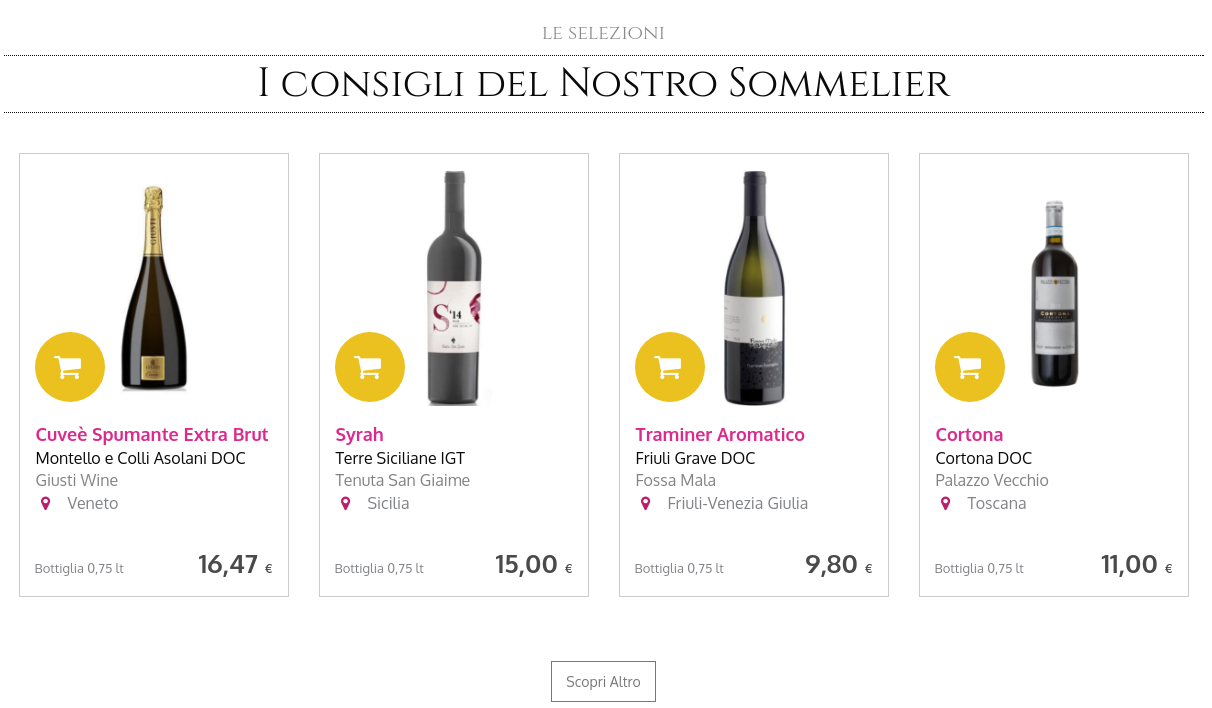
\includegraphics[width=\textwidth]{figure/oprod.png}
  \caption{Contenuto mostrato dal widget "Origni - Slider prodotti".}
  \label{fig:oprod}
\end{figure}


% ---------------- Origini - Banda tuttoschermo ----------------
\newpage
\section{Origini - Banda tuttoschermo}
Il Widget "Origini - Banda tuttoschermo" visualizza quella porzione di HTML
usata attualmente per lo "Speciale regione" (vedi Figure \ref{fig:oreg}).

Il form permette di modificare i seguenti campi (riferirsi a Figure \ref{fig:oreg}):
\begin{itemize}
\item Sottotitolo: il testo "Speciale regione"
\item Titolo: il testo "Lombardia e cultura del buon vino"
\item Descrizione: il testo della descrizione "La varietà dei territori..."
\item Link: l'URL a cui punta il tasto \emph{Scopri Altro}
\item Image-Link: l'URL dell'immagine di sfondo
\end{itemize}

\begin{figure}
  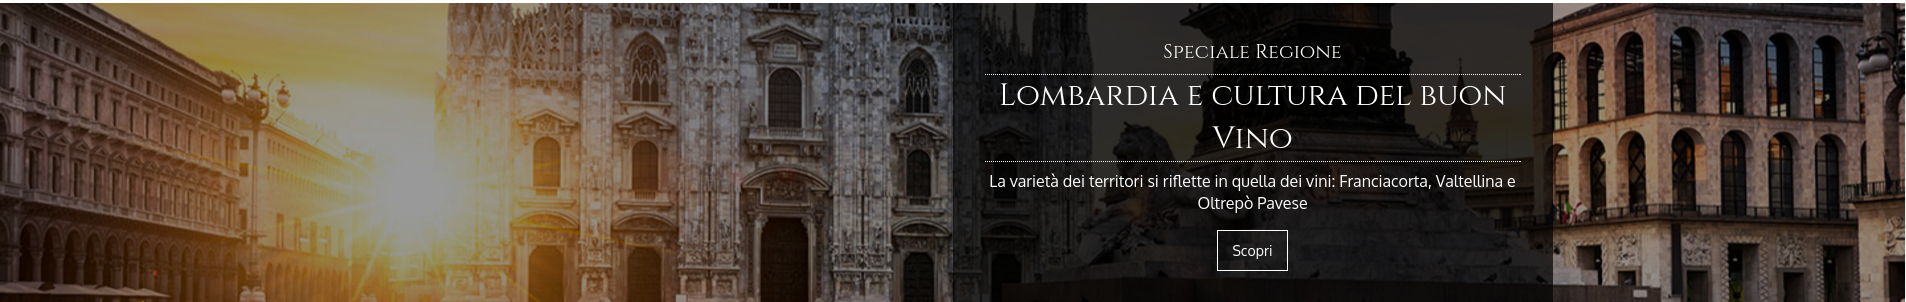
\includegraphics[width=\textwidth]{figure/oreg.png}
  \caption{Contenuto mostrato dal widget "Origni - Banda tuttoschermo".}
  \label{fig:oreg}
\end{figure}

% ---------------- Origini - Speciale ----------------
\newpage
\section{Origini - Speciale}
Il Widget "Origni - Speciale" visualizza quella porzione di HTML
usata attualmente per lo "Speciale del mese" (vedi Figure \ref{fig:ospec}).

Il form permette di modificare i seguenti campi (riferirsi a Figure \ref{fig:ospec}):
\begin{itemize}
\item Sottotitolo: il testo "La cantina del mese"
\item Titolo: il testo "Federico Ferrero"
\item Descrizione: il testo della descrizione "L’azienda agricola Ferrero nasce..."
\item Link: l'URL a cui punta il tasto \emph{Scopri Altro}
\item Image-Link: l'URL dell'immagine da visualizzare
\end{itemize}

\begin{figure}
  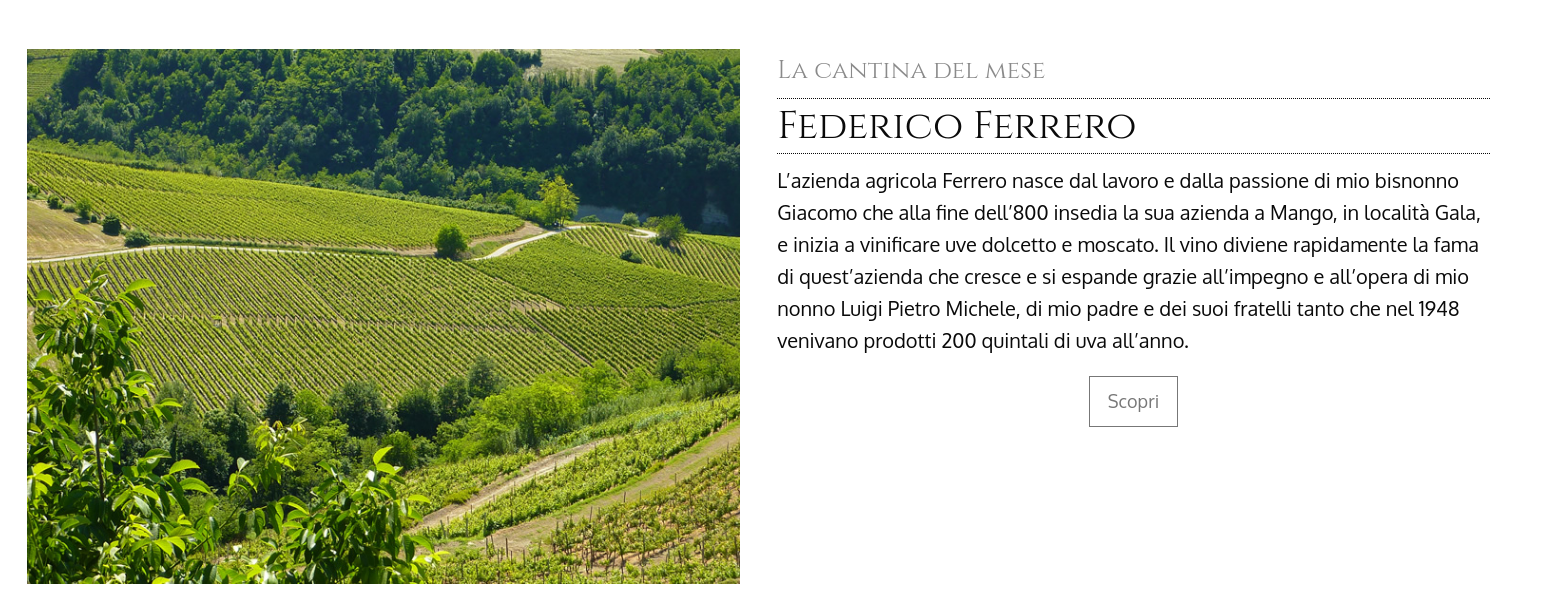
\includegraphics[width=\textwidth]{figure/ospec.png}
  \caption{Contenuto mostrato dal widget "Origni - Speciale".}
  \label{fig:ospec}
\end{figure}


  
%-------------------------------------------------------------
%       WIDGET ORIGINI
%-------------------------------------------------------------

\mcchap{Widgets di Kirivo}{cap:w-k}


%-------------------------------------------------------------
%       WIDGET KIRIVO
%-------------------------------------------------------------

\newpage

% ---------------- Kirivo - Immagini Speciali ----------------

\section{Kirivo - Immagini Speciali}

Il Widget "Kirivo - Immagini Speciali" permette di modificare il contenuto
delle prime due immagini della Homepage, ovvero le immagini solitamente dedicate
allo speciale del mese e alle offerte 

I campi che si possono modificare sono (riferirsi a Figura \ref{fig:kspec}):
\begin{itemize}
\item Link speciale: l'URL dove si viene indirizzati quando si schiaccia sull'immagine dello speciale
\item Url immagine speciale desktop: l'url dell'immagine da mettere nello speciale per desktop
\item Url immagine speciale mobile: l'url dell'immagine da mettere nello speciale per mobile
\item Link offerte: l'URL dove si viene indirizzati quando si schiaccia sull'immagine delle offerte
\item Url offerte speciale desktop: l'url dell'immagine da mettere nelle offerte per desktop
\item Url offerte speciale mobile: l'url dell'immagine da mettere nelle offerte per mobile
\end{itemize}

\begin{figure}
  
\includegraphics[width=\textwidth]{figure/kspec.png}
  \caption{Contenuto mostrato dal widget "Kirivo - Immagini Speciali".}
  \label{fig:kspec}
\end{figure}

% ---------------- Kirivo - Immagini Newsletter ----------------

\newpage
\section{Kirivo - Immagini Newsletter}

Il Widget "Kirivo - Immagini Newsletter" permette di modificare il contenuto
delle prime due immagini della Homepage, ovvero le immagini solitamente dedicate
allo speciale del mese e alle offerte 

I campi che si possono modificare sono (riferirsi a Figura \ref{fig:knews}):
\begin{itemize}
\item Url immagine newsletter desktop: l'url dell'immagine da mettere nella sezione "iscriviti alla newsletter"
\item Url immagine newsletter mobile: l'url dell'immagine da mettere nella sezione "iscriviti alla newsletter"
\item Link offerta: l'URL dove si viene indirizzati quando si schiaccia sull'immagine dell'offerta
\item Url offerta desktop: l'url dell'immagine da mettere nelle offerta per desktop
\item Url offerta mobile: l'url dell'immagine da mettere nelle offerta per mobile
\end{itemize}

\begin{figure}
  
\includegraphics[width=\textwidth]{figure/knews.png}
  \caption{Contenuto mostrato dal widget "Kirivo - Immagini Newsletter".}
  \label{fig:knews}
\end{figure}

% ---------------- Kirivo - Prodotti in evidenza ----------------

\newpage
\section{Kirivo - Prodotti in evidenza}

Il Widget "Kirivo - Prodotti in evidenza" visualizza quella porzione di HTML usata
per visualizzare i prodotti in evidenza (vedi Figura \ref{fig:kevid}).

I campi che si possono modificare sono (riferirsi a Figura \ref{fig:kevid}):
\begin{itemize}
\item Titolo: il testo "PRODOTTI IN EVIDENZA".
\item Ids: l'ID dei prodotti da visualizzare separati da virgola. I prodotti devono
essere almeno tre, se sono più di tre verranno usati i primi 3 ID validi.
\end{itemize}

\begin{figure}
  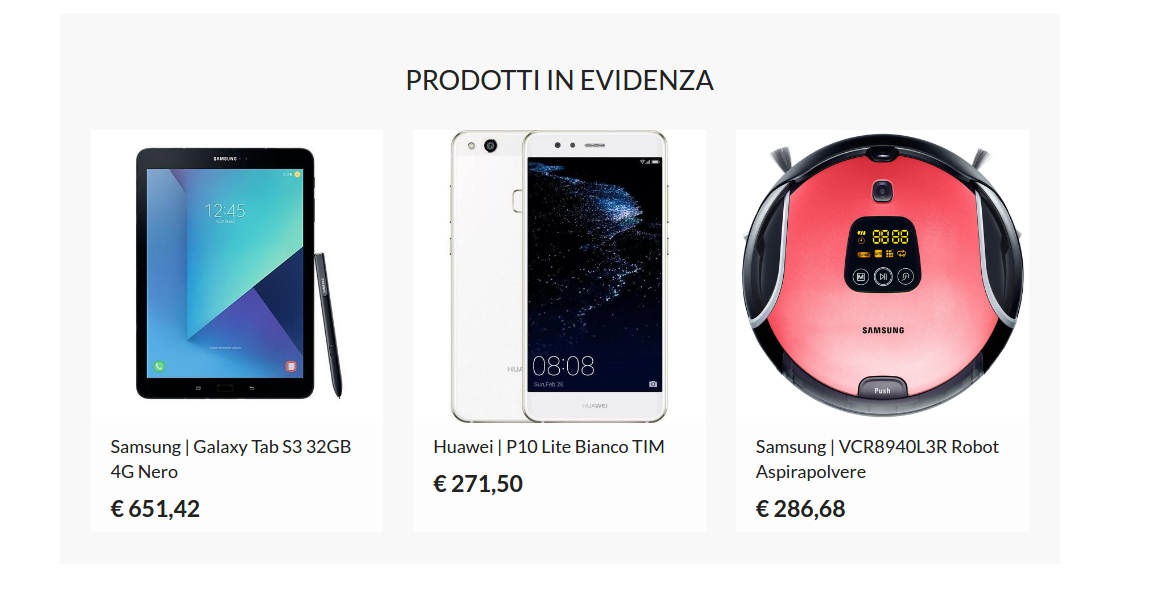
\includegraphics[width=\textwidth]{figure/kevid.png}
  \caption{Contenuto mostrato dal widget "Kirivo - Prodotti in evidenza".}
  \label{fig:kevid}
\end{figure}

\newpage
\section{Kirivo - Slider prodotti}

% ---------------- Kirivo - Slider prodotti ----------------

Il Widget "Kirivo - Slider prodotti"   visualizza quella porzione di HTML usata
per visualizzare uno slider di un insieme di prodotti (vedi Figura \ref{fig:kslide}).

I campi che si possono modificare sono (riferirsi a Figura \ref{fig:kslide}):
\begin{itemize}
\item Titolo: il testo "PRODOTTI PIÙ POPOLARI".
\item Numero max: il numero massimo di prodotti da visualizzare. Se lasciato vuoto non viene imposto alcun limite.
\item Ids: l'ID dei prodotti da visualizzare separati da virgola. I prodotti devono
essere almeno quanti specificati in numero max o quattro se non viene specificato.
\end{itemize}

\begin{figure}
  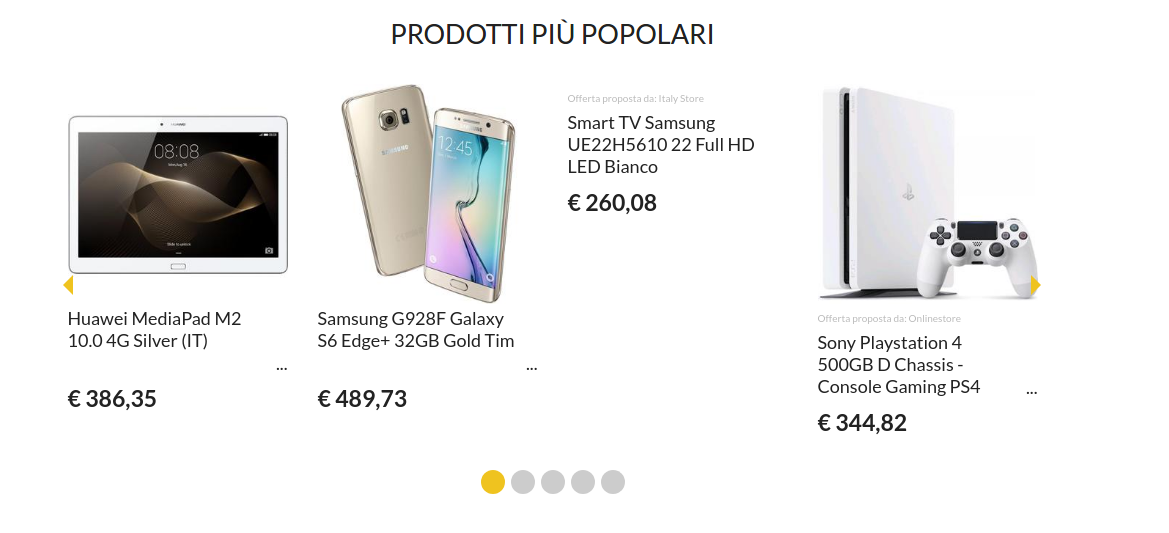
\includegraphics[width=\textwidth]{figure/kslide.png}
  \caption{Contenuto mostrato dal widget "Kirivo - Slider prodotti".}
  \label{fig:kslide}
\end{figure}


%%inserisci qui i tuoi capitoli
  
  \appendix
  %%%%%%%%%% CAPITOLO DI TESI %%%%%%%%%%
%
% Colophon 
%
%%%%%%%%%%%%%%%%%%%%%%%%%%%%%%%%%%%%%%
\chapter*{Colophon}

La tesi è stata scritta utilizzando il linguaggio LaTeX.\\
Le immagini sono state create appositamente usando screenshots delle applicazioni ed eventualmente editate con GIMP.\\


\backmatter{}

%% Bibliografia
  
  \printindex
  \bibliographystyle{bibliografia/IEEEtran}
  \bibliography{bibliografia/IEEEabrv,bibliografia/biblio}
   
\end{document}
